\documentclass[Main]{subfiles}

\begin{document}
\chapter{Lagrangian Systems and Pierels Brackets}
   %introduzione


	\section{Abstract Lagragian Systems}
	%Definizione deI sistemi Lagrangiani in Astratto
	
	\begin{definition}[Lagrangian System]
	Pair $(E, \mathcal{L} )$ composed of:
		\begin{itemize}
			\item $E \xrightarrow{\pi} M$ smooth fiber bundle of typical fiber $Q$ called \emph{"configuration bundle"}.
			\item	$ \mathcal{L} : J^r E \rightarrow \Omega^m (M)$ function from the r-th Jet Bundle to  the top-dimensionial form over the base manifold $M$  called \emph{"Lagrangian density"} or simply \emph{"Lagrangian"} of r-th order.
		\end{itemize}
	\end{definition}	
	
	
	\subsection{Kinematics}
	%Fibrato Configurazione incompassa la cinematica
	The configuration bundle encompass all the kinematical structure of the system, the pivotal role is played by the smooth sections  which are to be understood as all the possible conformation of the system.

	\begin{notationfix}
		\begin{displaymath}
			\Conf= \Gamma^\infty(M,E)
		\end{displaymath}
		Space of kinematic configurations.
	\end{notationfix}

	A section is not a statical configuration, equivalent to a specific point in the configuration space of ordinary classical systems, but has to be seen as a specific realization of the kinematics in the sense of  a complete description of a possible motion.
	At this level of abstraction, since no space-time structure has been specified, terms like stasis and motion must be taken with care .The natural physical interpretation should be clearly manifested through the concrete realization of systems with discrete and continuous degree of freedom.
	
	\begin{observation}[Mathematical structure]
	Mathematically speaking this set should be regarded as an infinite dimensional Manifold. 
	
	This framework provides a geometric characterization of the notion of variations as tangent vectors on the the space of kinematic configurations .\cite{Forger2005}
	\end{observation}
	
	\begin{observation}[Coordinate Representation]
	The choice of a chart atlas $\Atlas(M)$ on the base space $M$ and $\Atlas(E)$ on the total space $E$ provides a correspondence between each configuration $\gamma \in \Conf$ and family of smooth real functions $\{f_{\alpha \beta}:A_\alpha \subset \Real^m \rightarrow \Real^q \}$.
	The process is trivial:
	\begin{displaymath}
		\gamma \in \Conf \mapsto \{f_{A,U}=\psi_U \circ \gamma \circ \psi_A^{-1} \vert (A,\psi_A) \in \Atlas(M), (U,\psi_U)\in \Atlas(E)   \}
	\end{displaymath}
	
	%	$\forall (A,\psi_A)$ local chart on $M$ and $(U,\psi_U)$ local chart on $E$ such that $\gamma(A) \cap U \neq \emptyset$ $f_{A,U}=\psi_U \circ \gamma \circ \psi_A^{-1}$

	Since the whole section as a global object is quite difficult to handle is customary in field theory to work in the more practical local representation. 
	\end{observation}	
	
	\begin{observation}[Further specification of the system's kinematics]
	 	The general formalism doesn't require any other structure to be carried forward.
	 	Additional structure on the fiber and the whole bundle are to be prescribed in order to specify a precise physical model, e.g. the spin structure for the Dirac Field.\cite{Benini}
	 \end{observation}	
	
	\begin{figure}[h!]
 	 	\caption{Geometric picture of the basic kinematic structure.}
   		%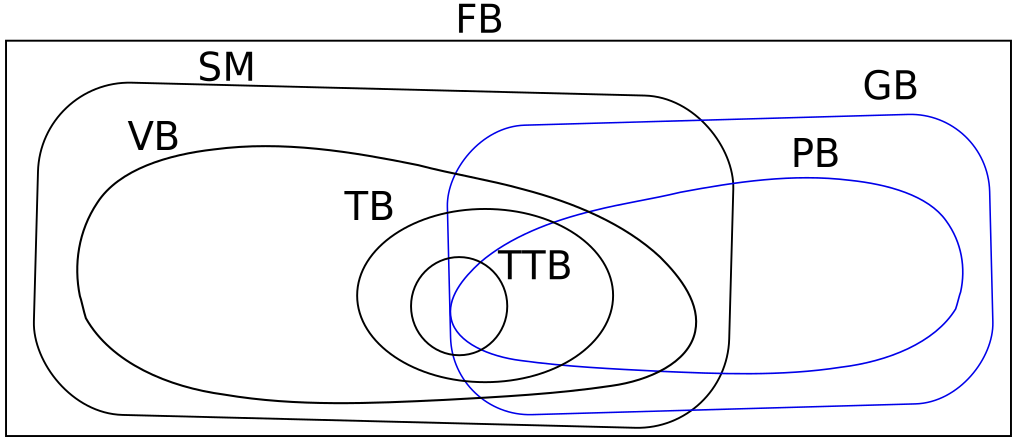
\includegraphics[width=0.5\textwidth]{Pictures/EuleroVenn_Bundles} 
  		\centering
	\end{figure}	
	
	\subsection{Dynamics}
	%la lagrangiana incompassa la dinamica
	
	%la classe delle densità lagrangiane
	
	%il funzionale lagrangiana totale e azione
	
	%Principio di minima azione e operatore delle equazioni del moto
	
	%Spazio delle configurazioni di Campo
	
	
	
	\subsection{Generalization}
	%Sistemi evolutivi e sistemi hamiltoniani	
	
%-_-_-_-_-_-_-_-_-_-_-_-_-_-_-_-_-_-_-_-_-_-_-_-_-_-_-_-_-_-_-_-_-_-_-_-_-_-_-_-_-_-_-_-_-_-_-_-_-_-_-_-_-_-_-_
\newpage
	\section{Concrete Realization}
	%esibiamo quanto è ampia la nostra definizione
		\subsection{Fields on curved Background}
		%M è spazio tempo,
		%bundle è lineare per prevedere il principio di sovrapposizione
		%M è glob iper e P è green iper per tener conto del comporatamento propagativo
		\subsection{Finite Degree systems}
		  % il fibrato non è vettoriale
		  % le configurazioni sono curve
		  % 
		
%-_-_-_-_-_-_-_-_-_-_-_-_-_-_-_-_-_-_-_-_-_-_-_-_-_-_-_-_-_-_-_-_-_-_-_-_-_-_-_-_-_-_-_-_-_-_-_-_-_-_-_-_-_-_-_
\newpage
	\section{Geometric mechanics of Finite Degree systems}
	%L'approccio usato generalmente è deduttivo dal particolare al generale
	%parlare di spazio delle fasi, forma simplettica, legendre
	%osservabili classici parentesi di poisson
	
	\subsection{Linear dynamical systems}	
	
%-_-_-_-_-_-_-_-_-_-_-_-_-_-_-_-_-_-_-_-_-_-_-_-_-_-_-_-_-_-_-_-_-_-_-_-_-_-_-_-_-_-_-_-_-_-_-_-_-_-_-_-_-_-_-_
\newpage
	\section{Peierls Brackets}
	%peierels vs poisson (sharan)
	
	\subsection{Finite Dimensional case}
	
%-_-_-_-_-_-_-_-_-_-_-_-_-_-_-_-_-_-_-_-_-_-_-_-_-_-_-_-_-_-_-_-_-_-_-_-_-_-_-_-_-_-_-_-_-_-_-_-_-_-_-_-_-_-_-_
\newpage
	\section{Eliminata}
	\begin{itemize}
		\item quando parlo della cinematica mi piacerebbe dare indicazioni sulla struttura matematica dello spazio delle configurazioni cinematiche:
			\begin{enumerate}
				\item costituisce una frechet manifold ( gli unici risultati che ho trovato sono quelli di Palais di "non linear global analysis"
				\item le curve parametrizzate sono le variazioni
				\item classi di equivalenza definiscono delle variazioni infinitesime che costituiscono lo spazio tangente allo spazio delle configurazioni cinematiche
				\item questo spazio tangente è isomorfo allo spazio delle sezioni del pullback rispetto alla sezione $\phi\in C$ del verical bundle (vedere forger romero)
				\item il problema dell'atlante e della rappresentazione delle sezioni in carta locale ( da scegliere sia sul total space E che sul base space M)
			\end{enumerate}
	\end{itemize}
	
\end{document}